\documentclass{VUMIFInfBakalaurinis}
\usepackage{algorithmicx}
\usepackage{algorithm}
\usepackage{algpseudocode}
\usepackage{amsfonts}
\usepackage{amsmath}
\usepackage{bm}
\usepackage{caption}
\usepackage{color}
\usepackage{float}
\usepackage{graphicx}
% \usepackage{hyperref}  % Nuorodų aktyvavimas
\usepackage{listings}
\usepackage{subfig}
\usepackage{url}
\usepackage{wrapfig}
\usepackage{tabularx}
\usepackage{booktabs}
\usepackage{array}% http://ctan.org/pkg/array

% Titulinio aprašas
\university{Vilniaus universitetas}
\faculty{Matematikos ir informatikos fakultetas}
\institute{Informatikos institutas}  % Užkomentavus šią eilutę - institutas neįtraukiamas į titulinį
\department{Informatikos katedra}
\papertype{Baigiamasis bakalauro darbas}
\title{Daiktų interneto prietaisų informacinė sistema}
\titleineng{Internet of things information system}
\status{4 kurso 2 grupės studentas}
\author{Šarūnas Ramanauskas}
% \secondauthor{Vardonis Pavardonis}   % Pridėti antrą autorių
\supervisor{dr. Igor Katin}
% \reviewer{doc. dr. Vardauskas Pavardauskas}
\date{Vilnius \\ \the\year}

% Nustatymai
% \setmainfont{Palemonas}   % Pakeisti teksto šriftą į Palemonas (turi būti įdiegtas sistemoje)
\bibliography{bibliografija} 

\begin{document}
\maketitle

\tableofcontents

\sectionnonum{Įvadas}

Sąvoka daiktų internetas (angl. Internet of Things – IoT) atsirado gana atsitiktinai.
Ją 1999 metais pirmą kartą konferencijos metu panaudojo mokslinių tyrimų grupės „Auto-ID Labs“ tuometinis vykdomasis direktorius Kevinas Ashtonas.

„Jeigu turėsime kompiuterius, kurie gebės surinkti bei panaudoti informaciją apie mus supančius daiktus be mūsų įsikišimo,
galėsime ne tik ženkliai sumažinti kasdieninį eikvojimą, bet taip pat gebėsime veikti produktyviau ir našiau.“
– 1999 metais pristatymo „Procter \& Gamble“ metu teigė Kevinas Ashtonas.

Pradinė idėja buvo siejama su radijo dažnio identifikavimo technologija RFID (angl. Radio-Frequency Identification).
Vis dėlto jau tada buvo aišku, jog daiktų internetas turi tapti tuo pagalbininku, padėsiančiu žmonėms apdoroti,
analizuoti bei panaudoti nuolatos augantį skaitmeninių duomenų srautą.
Kitaip sakant, nuo pat pirmosios akimirkos visuomenei buvo bandoma pasakyti,
kad daiktų internetas ruošiasi modernizuoti buitį bei mus supančiam inventoriui suteikti „protą“.

Įsivaizduokite, ryte suskambęs žadintuvas virtuvėje stovinčiam kavos aparatui liepia paruošti kavą,
o darbo kambaryje stovintis spausdintuvas pats seka spausdinimui skirtų lapų likutį bei atėjus metui automatiškai
pasirūpina jų užsakymu iš parduotuvės. Lygiai taip pat galėtų elgtis reikalaujamą maistą be žmogaus įsikišimo į namus užsakantis
išmanusis šaldytuvas. Akivaizdu, daiktų internetas gali plėtoti autonominius skaitmeninius duomenų transporto tinklus,
kurie padėtų kurti ir įgyvendinti visavertę išmaniųjų namų, gamyklų bei miestų idėją.

Kita vertus, integruoti didelio našumo procesorius į kiekvieną buityje naudojamą prietaisą yra nepraktiška. Daiktų interneto prietaisai susideda
iš dviejų esminių komponentų - sensorių ir valdiklių. Sensorius fiksuoja atitinkamus paties įrenginio arbo jo aplikos duomenis ar parametrus.
Valdiklis skirtas prietaiso funkcijoms aktyvuoti. Prietaiso fiksuojamų duomenų apdorojimas ir jo valdiklių aktyvavimas gali vykti centralizuotai taip sujungiant 
daug skirtingų prietaisų į bendrą tinklą. Įrenginys savaime geba tik išsiųsti savo surinktus duomenis, priimti ir įvykdyti funkcijas kurioms jis buvo sukurtas.
Iš šio konteksto kylantis uždavinys - reikalinga programinė įranga suteikianti galimybę valdyti interneto daiktų prietaisus, rinkti ir stebėti jų renkamus duomenis.

\par Šio darbo tikslas - sukurti daiktų interneto valdymo sistemos prototipą.
Uždaviniai:
\begin{itemize}
  \item Išnagrinėti dalykinę sritį. Atlikti panašių, daiktų interneto prietaisus administruojančių, informacinių sistemų analizę ir palyginimą.
  \item Sukurti universalios daiktų interneto prietaisų informacinės sistemos projektą. Atlikti reikalavimų ir projektavimo specifikacijas.
  \item Išrinkti programavimo technologijas skirtas vartotojo sąsajos, duomenų saugojimo ir apdorojimo komponentų kūrimui.
  \item Realizuoti universalios informacinės sistemos projektą, skirtą administruoti daiktų interneto prietaisus.
\end{itemize}

\section{Daiktų internetas}
Daiktų internetas (angl. Internet of things - IOT) apibūdina fizinių objektų - „daiktų“ ar objektų - tinklą, įterptą su jutikliais, programine įranga ir kitomis technologijomis, siekiant prisijungti ir keistis duomenimis su kitais prietaisais 
ir sistemomis internete. Pagrindą tam suteikė realaus laiko analizės, mašininio mokymosi, jutiklių ir įterptųjų sistemų vystymasis. Tradiciniai įterptųjų sistemų, belaidžių jutiklių tinklų, valdymo sistemų, 
automatikos (įskaitant namų ir pastatų automatizavimą) ir kitos taikymo sritys prisideda prie daiktų interneto įgalinimo. Vartotojų rinkoje daiktų interneto technologija yra labiausiai sinonimas produktams,
susijusiems su „protingo namo“ sąvoka, įskaitant prietaisus ir įrenginius (tokius kaip šviestuvai, termostatai, namų apsaugos sistemos ir kameros bei kiti buitiniai prietaisai).
Yra daug rimtų susirūpinimų dėl DI augimo pavojų, ypač privatumo ir saugumo srityse, todėl pramonės ir vyriausybės ėmėsi veiksmų šiems susirūpinimams spręsti, įskaitant tarptautinių standartų kūrimą.

\subsection{Istorija}
Pagrindinė išmaniųjų įrenginių tinklo koncepcija buvo aptarta jau 1982 m.,
Kai modifikuotas „Coca-Cola“ pardavimo automatas Carnegie Mellon universitete tapo pirmuoju prie interneto prijungtu prietaisu, galinčiu pranešti apie savo atsargas ir tai, ar naujai pakrauti gėrimai buvo šalti, ar ne.
1991 m. Marko Weiserio straipsnis apie visur esančią kompiuteriją „XXI amžiaus kompiuteris“, taip pat tokios akademinės vietos kaip „UbiComp“ ir „PerCom“ sukūrė šiuolaikinę "IOT" viziją. 1994 m.
Reza Raji apibūdino šią sąvoką kaip „perkelti mažus duomenų paketus į didelį mazgų rinkinį, kad būtų galima integruoti ir automatizuoti viską, pradedant buitine technika ir baigiant visomis gamyklomis“.
1993–1997 m. bendrovės „Microsoft“ ir „Novell“ pasiūlė pirmuosius daiktų interneto sistemų sprendimus. Ši sritis įgavo pagreitį, kai Billas Joy'as numatė, kad ryšys tarp prietaisų yra jo „Šeši tinklai“ sistemos dalis, pristatyta 
Pasaulio ekonomikos forume Davose 1999 m. Terminą „daiktų internetas“ sugalvojo Kevinas Ashtonas iš „Procter \& Gamble“, vėliau MIT „Auto-ID Center“, 1999 m., Nors jis labiau mėgsta frazę „Internetas“. 
Tuo metu jis laikė radijo dažnio identifikavimą (RDA) būtinu daiktų internetui, kuris leistų kompiuteriams valdyti visus atskirus dalykus. Apibrėždama daiktų internetą kaip „paprasčiausiai laiko momentą,
kai prie interneto prijungta daugiau„ daiktų ar objektų “nei žmonių“, „Cisco Systems“ apskaičiavo, kad daiktų internetas „gimė“ 2008–2009 m., Daiktų ir žmonių santykiui augant. nuo 0,08 2003 m. iki 1,84 2010 m. \cite{Technologijos}
\subsection{Taikymo sritys}

\subsubsection{Protingi namai}
DI prietaisai yra didesnės namų automatikos koncepcijos dalis, kuri gali apimti apšvietimą, šildymą ir oro kondicionavimą, laikmenų ir apsaugos sistemas bei kamerų sistemas.
Ilgalaikė nauda galėtų apimti energijos taupymą automatiškai užtikrinant, kad žibintai ir elektronika būtų išjungti, arba informuodami namų gyventojus apie jų naudojimą.
Protingi namai arba automatizuoti namai galėtų būti grindžiami platforma ar mazgais, kurie valdo išmaniuosius įrenginius ir prietaisus.
Pavyzdžiui, naudodamiesi „Apple HomeKit“ gamintojai savo namų produktus ir priedus gali valdyti taikydami „iOS“ įrenginių, tokių kaip „iPhone“ ir „Apple Watch“, programas.
Tai gali būti skirta programa arba „iOS“ vietinės programos, tokios kaip „Siri“.
Tai galima įrodyti „Lenovo Smart Home Essentials“ atveju - tai išmaniųjų namų įrenginių, valdomų per „Apple Home“ programą ar „Siri“, nereikalaujantis „Wi-Fi“ tilto, linija.
Taip pat yra specialių išmaniųjų namų centrų, kurie siūlomi kaip atskiros platformos, skirtos sujungti skirtingus išmaniųjų namų produktus.
Tai apima „Amazon Echo“, „Google Home“, „Apple HomePod“ ir „Samsung“ „SmartThings Hub“. Be komercinių sistemų, yra daugybė nepatentuotų, atviro kodo ekosistemų; įskaitant „Home Assistant“, „OpenHAB“ ir „Domoticz“. \cite{IOTWiki}

\subsubsection{Medicina ir sveikatos priežiūra}
The Medicinos daiktų internetas (IoMT) yra daiktų interneto taikymas medicinos ir sveikatos tikslais, tokais kaip duomenų rinkimas ir analizė medicininiams tyrimams arba pacientų stebėsena.
IoMT buvo vadinama „išmaniąja sveikatos priežiūra“, kaip technologija, skirta sukurti skaitmeninę sveikatos priežiūros sistemą, susieti turimus medicinos išteklius ir sveikatos priežiūros paslaugas.
DI prietaisai gali būti naudojami nuotolinio sveikatos stebėjimo ir pranešimo apie ekstremalias situacijas sistemoms įgalinti.
Šie sveikatos stebėjimo prietaisai gali būti nuo kraujo spaudimo ir širdies ritmo monitorių iki pažangių prietaisų, galinčių stebėti specializuotus implantus, tokius kaip širdies stimuliatoriai, „Fitbit“ elektroninės riešinės ar pažangiosios klausos priemonės.
Kai kurios ligoninės pradėjo diegti „išmaniąsias lovas“, kurios galėtų nustatyti, kada jos yra užimtos ir kada pacientas bando keltis.
Taip pat esama prietaisų, galinčių prisitaikyti prie paciento poreikių, pavydžiui, užtikrinančių tinkamą spaudimą ir palaikymą pacientui be slaugytojų priežiūros.
2015 m. „Goldman Sachs“ ataskaita nurodė, kad sveikatos priežiūros IoT prietaisai „gali sutaupyti Jungtinėms Valstijoms daugiau nei 300 mlrd. USD metinių sveikatos priežiūros išlaidų, didinant pajamas ir mažinant išlaidas“.
Be to, naudojant mobiliuosius prietaisus medicininei veiklai buvo sukurta „m-sveikata“, naudojama sveikatos statistikos analizei.
Gyvenamosiose patalpose taip pat gali būti įrengti specializuoti jutikliai, skirti stebėti pagyvenusių žmonių sveikatą ir bendrą savijautą, taip pat užtikrinant, kad būtų skiriamas tinkamas gydymas,
taip pat padedant žmonėms atgauti prarastą judrumą gydant. Šie jutikliai sukuria intelektualių jutiklių tinklą, galintį rinkti, apdoroti, perduoti ir analizuoti vertingą informaciją įvairiose aplinkose,
pavyzdžiui, prijungti stebėjimo namuose įrenginius prie ligoninėse veikiančių sistemų. Kiti vartojimo prietaisai, skatinantys sveiką gyvenimo būdą, pvz., Prijungtos svarstyklės ar nešiojami širdies monitoriai, taip pat yra IoT galimybė.
Priešgimdyminiams ir lėtiniams pacientams taip pat yra prieinamos sveikatos stebėjimo sistemos, užtikrinančios sveikatos būklę ir pasikartojančius vaistų poreikius.
Nuo 2018 m IoMT buvo taikomas ne tik klinikinių laboratorijų pramonėje, bet ir sveikatos priežiūros bei sveikatos draudimo pramonėje.
IoMT sveikatos priežiūros pramonėje dabar leidžia gydytojams, pacientams ir kitiems asmenims, tokiems kaip pacientų globėjai, slaugytojai, šeimos ir panašūs, būti sistemos dalimi, kai pacientų įrašai saugomi duomenų bazėje,
leidžiančioje gydytojams ir likusiems žmonėms medicinos personalui suteikti prieigą prie pacientų informacijos. Be to, IoT pagrįstos sistemos yra orientuotos į pacientą, o tai reiškia, kad pacientas turi būti lankstus atsižvelgiant į sveikatos būklę.
Draudimo srityje esanti IoMT suteikia prieigą prie geresnės ir naujos rūšies dinamiškos informacijos. Tai apima jutikliais pagrįstus sprendimus, tokius kaip biosensoriai, nešiojamieji kompiuteriai, prijungti sveikatos priežiūros prietaisai
ir mobiliosios programos klientų elgsenai stebėti. DI taikymas sveikatos priežiūros srityje vaidina pagrindinį vaidmenį valdant lėtines ligas, taip pat prevencijai ir kontrolei.
Nuotolinis stebėjimas yra įmanomas sujungus galingus belaidžius sprendimus. Ryšys leidžia sveikatos priežiūros specialistams užfiksuoti paciento duomenis ir taikyti sudėtingus algoritmus sveikatos duomenų analizėje.
\cite{IOTWiki}

\subsubsection{Transportas}
DI gali padėti integruoti ryšius, valdyti ir apdoroti informaciją įvairiose transporto sistemose.
DI taikomas visiems transporto sistemų aspektams (t. y. Transporto priemonei, infrastruktūrai ir vairuotojui ar naudotojui). Dinaminė šių transporto sistemos komponentų sąveika suteikia galimybę susisiekti transporto priemonėse, 
išmaniai valdyti eismą, statyti automobilius. Taip pat daiktų interneto spendimai gali būti taikomi elektroninėse rinkliavų surinkimo sistemose, automobilių parkų valdyme, siekiant pagerinti eismo saugumą ir pagalbos kelyje efektyvumą.

%\subsubsection{Gamyba ir Žemdirbystė}
%Daiktų internetas gali prijungti įvairius gamybos įrenginius ir gamybos linijas, kuriose įdiegtos jutimo, identifikavimo, apdorojimo, ryšio, valdymo ir tinklo galimybės.
%Gamybos operatoriai gali sklandžiai stebėti visą gamybos linijos darbą ir greitai pastebėti ir imtis veiksmų esant neskalndumams. Tai didna gamybos procesų našumą ir gaminamos produkcijos kokybę.
%
%Žemės ūkyje yra daugybė daiktų interneto, pavyzdžiui, gali rinkti duomenis apie temperatūrą, kritulius, drėgmę, vėjo greitį, kenkėjų užkrėtimą ir dirvožemio kiekį.
%Šie duomenys gali būti naudojami ūkininkavimo metodams automatizuoti, priimti pagrįstus sprendimus siekiant pagerinti kokybę ir kiekį, sumažinti riziką ir švaistymą bei sumažinti pasėlių valdymui reikalingas pastangas.
%Pavyzdžiui, ūkininkai dabar gali iš tolo stebėti dirvožemio temperatūrą ir drėgmę ir net pritaikyti IoT gautus duomenis tiksliojo tręšimo programoms.
%\cite{IOTWiki}

\subsection{Daiktų interneto ekosistema}

Bendruoju atveju apibrėžiant daiktų internetą, visose jo taikymo srityse galima išskirti šias pagrindines sudedamasias dalis:

\begin{itemize}
  \item \emph{Prietaisai} - smulkiausias daiktų interneto vienetas. Įrenginys gebantis rinkti duomenis ir/arba vykdyti savo funkciją(-as).
  \item \emph{Tinklo sistemos(Internetas)} - infrastruktūra skirta įrenginių sujungimui į bendrą tinklą. Norint įgalinti įrengius jiems reikalnga prieiga prie viešo arba vietinio interneto tinklo. 
  \item \emph{Debesis} - Taikomosios stebėjimo ir valdymo programos. Sprendimai renkamų duomenų saugojimui, analizei, įrenginių stebėjimui ir valdymui.
\end{itemize}

Šios trys dalys įvardijamos kaip pagrindiniai daiktų interneto architektūros sluoksniai. \cite{IOTR, IOTV}

\begin{figure}[H]
    \centering
    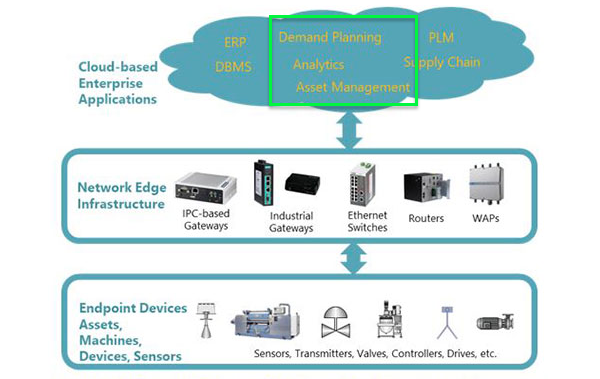
\includegraphics[scale=0.6]{img/iot-high-level}
    \caption{Daiktų interneto ekosistema}   % Antraštė įterpiama po paveikslėlio
    \label{img:mlp}
\end{figure}

Informacinės sistemos skirtos daiktų interneto įrenginių stebėjimui ir valdymui patenka į trečiąjį sluoksnį(žr. pav.).
Kaip jau aprašyta pirmame skyriuje, daiktų internetas turi labai daug taikymo sričių, kuriose skirtingiems tiklsams naudojami skirtingi įrenginiai.
Iš to išplaukia vienas esminių informacinės sistemos reikalavimų - sistema turi sugebėti palaikyti įvairius įrenginius, priimti skirtingus duomenis siunčiamus iš skirtingo tipo įrenginių.
Taip pat kiekvienas įrenginys turi sau specifinę konfigūraciją, kurios valdymas ir keitimas gali būti vykdomas informacinės sistemos pagalba.
Svarbus aspektas yra įrenginių skaičius. Pavydžiui, vien namuose galima įdiegti didelį skaičių daiktų interneto prietaisų. Kiekviename namo kambaryje gali buti atskiri temperatūros davikliai, šviesos jungikliai, langų žaliuzių valdikliai ir taip toliau.
\par Į grupes sujungti įrenginiai gali veikti kaip vientisa sistema. Pavydžiui, gamybos linijoje esantys sensoriai siunčia informaciją apie žaliavų kiekį ir priklausomai nuo to sistemos administratorius turi gebėti koreguoti kitų gamybos linijoje esančių įrenginių būseną(konfigūraciją). 

\par Taigi, pagrindiniai sistemos kriterijai:
\begin{itemize}
  \item \emph{Prietaisai} - sistema turi gebėti palaikyti įvairius įrenginius, priimti skirtingus duomenis siunčiamus iš skirtingo tipo įrenginių. Taip turi būti numatyta galimybė dinamiškai
  apibrėžti įrenginio konfigūraciją.
  \item Įrenginių tinklas gali susideti iš didelio skaičiaus prietaisų. Sistemoje turi būti numatyta galimybė skirstyti prietaisus į grupes pagal jų lokaciją arba paskirtį.
  \item Kiekvieno įrenginio būsenos stebėjimas ir nustatymų keitimas yra žmogaus įsiterpimo ir laiko reikalaujantis procesas.
    Reikalinga įgyvendinti sprendimą leidžiantį sukonfigūruoti scenarijus kai sistema automatiškai pakeičia įrenginio(arba kitų įrenginių) konfigūraciją priklausomai nuo surenkamų duomenų.
\end{itemize}


\subsection{Egzistuojančių sprendimų analizė}

\subsubsection{Kaa IoT}
„Kaa“ yra visapusiška daiktų interneto platforma, taikoma bet kokio masto įmonės daiktų interneto projektams. Ji siūlo daugybę funkcijų, leidžiančių kūrėjams kurti pažangias programas išmaniesiems produktams,
lanksčiai valdyti savo prijungtus įrenginius per debesį, organizuoti visišką duomenų apdorojimą, analizuoti įrenginio telemetriją ir dar daugiau. Su IoT funkcijomis, kurias „Kaa“ teikia,
galima kurti savo IoT programas iki 10 kartų greičiau nei anksčiau.
Visos „Kaa“ funkcijos yra įdiegtos naudojant mikro servisus, o „Kaa“ visuma yra pagrįsta lanksčia mikro servisų architektūra.
Tai reiškia, kad galima atskirai tinkinti kiekvieną Kaa funkciją, pridėti naujų arba esamas pakeisti kai kuriais trečiųjų šalių įrankiais.
„Kaa“ siūlo visas daiktų interneto funkcijas, kurių gali prireikti įprastai IoT programai – nuo ​​duomenų rinkimo ir įrenginių valdymo iki daiktų interneto prietaisų skydelių ir analizės.
Taip pat galite pasinaudoti atviromis API, kad integruotumėte Kaa funkcijas į savo modulius ir programas.
Šioje diagramoje parodyta bendra funkcinė Kaa architektūra.

\begin{figure}[H]
  \centering
  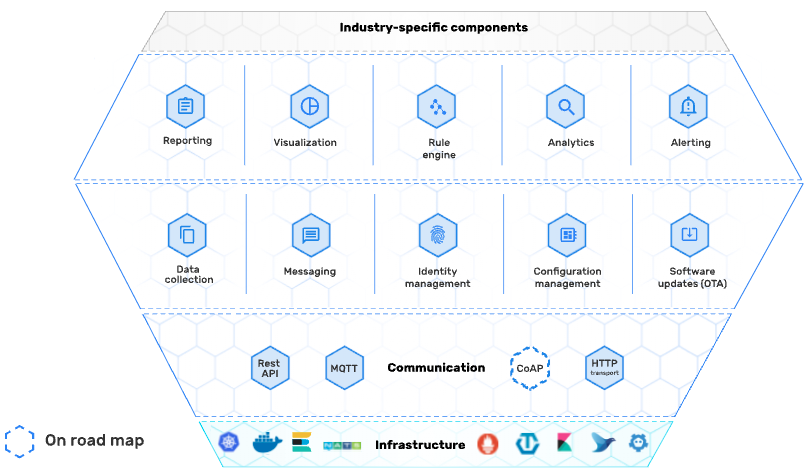
\includegraphics[scale=0.6]{img/kaa-arch}
  \caption{Kaa IoT platformos komponentai}   % Antraštė įterpiama po paveikslėlio
  \label{img:mlp}
\end{figure}

\subsubsection{ThingSpeak}
ThingSpeak™ yra IoT analizės platformos paslauga, leidžianti kaupti, vizualizuoti ir analizuoti tiesioginius duomenų srautus debesyje.
„ThingSpeak“ teikia įrenginių duomenų vizualizacijas. Turėdami galimybę vykdyti MATLAB® kodą ThingSpeak, galite atlikti internetinę duomenų analizę ir apdorojimą.
„ThingSpeak“ dažnai naudojama prototipams kurti ir IoT sistemoms, kurioms atliekama renkamų duomenų analizė.

\begin{figure}[H]
  \centering
  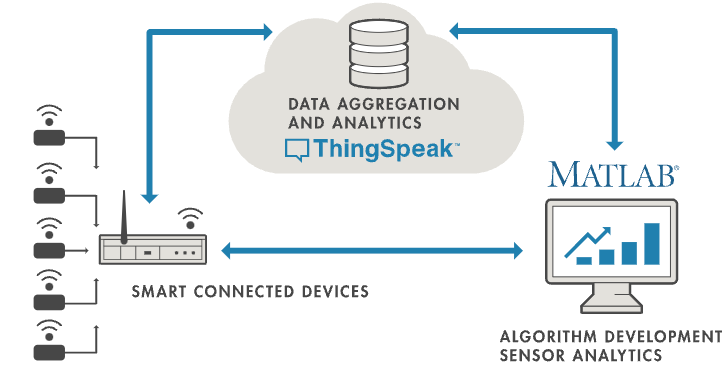
\includegraphics[scale=0.5]{img/thing-speak-arch}
  \caption{ThingSpeak platforma}   % Antraštė įterpiama po paveikslėlio
  \label{img:mlp}
\end{figure}

„ThingSpeak“ leidžia kaupti, vizualizuoti ir analizuoti tiesioginius duomenų srautus debesyje. Kai kurios pagrindinės ThingSpeak galimybės:

\begin{itemize}
\item Lengvai konfiūruoti įrenginius ir siųsti duomenis į ThingSpeak naudojantis populiariariais IoT protokolais.
\item Vizualizuoti jutiklio duomenis realiuoju laiku.
\item Apibendrinti duomenis pagal pareikalavimą iš trečiųjų šalių šaltinių.
\item Naudotis MATLAB, atlikti analitikos uždavinius su savo daiktų interneto duomenimis.
\item Automatiškai valdyti daiktų interneto prietaisus pagal tvarkaraščius ar įvykius.
\item Reakcijos į duomenis – tiek neapdorotus, tiek naujus, apskaičiuojamus, duomenis. Sistemoje apibrėžiamos taisyklės(\emph{Conditions}) ir veiksmai (\emph{Actions}) atliekami, kai taisyklės/sąlygos patenkinamos.
\end{itemize}

\subsubsection{AWS IoT Core}
„AWS IoT Core“ leidžia prijungti įrenginius prie AWS debesų kompiuterijos paslaugų ir kitų įrenginių, apsaugoti duomenis ir kurti jų tarpusavio sąveiką, apdoroti įrenginio duomenis ir veikti pagal juos,
leidžia programoms sąveikauti su įrenginiais.

AWS IoT Core galimybės:
\begin{itemize}
\item \emph{AWS IoT Device SDK} padeda lengvai ir greitai prijungti aparatūros įrenginį arba mobiliąją programą prie AWS IoT Core.
AWS IoT įrenginio SDK leidžia įrenginiams prisijungti, autentifikuotis ir keistis pranešimais su AWS IoT Core naudojant MQTT, HTTP arba WebSockets protokolus.
AWS IoT įrenginio SDK palaiko C, JavaScript ir Arduino ir apima klientų bibliotekas, kūrėjo vadovą ir perkėlimo vadovą gamintojams.
Taip pat galima naudoti atvirojo kodo alternatyvą arba parašyti savo SDK.

\item \emph{Device Gateway}
Tai yra IoT įrenginių, besijungiančių prie AWS, įėjimo taškas.
\emph{Device Gateway} valdo visus aktyvius įrenginių ryšius ir įgyvendina kelių protokolų semantiką, kad užtikrintų, jog įrenginiai galėtų saugiai ir efektyviai susisiekti su AWS IoT Core.

\item \emph{Rules Engine}
Taisyklių modulis leidžia kurti daiktų interneto programas, kurios renka, apdoroja, analizuoja ir veikia prijungtų įrenginių generuojamus duomenis.
Taisyklių modulis įvertina gaunamus pranešimus, paskelbtus AWS IoT Core, ir transformuoja bei pristato juos į kitą įrenginį arba debesies paslaugą pagal apibrėžtas verslo taisykles.
Taisyklė gali būti taikoma duomenims iš vieno ar kelių įrenginių ir lygiagrečiai gali atlikti vieną ar kelis veiksmus.
Taisyklių modulis taip pat gali nukreipti pranešimus į AWS galinius taškus, įskaitant AWS IoT Analytics, AWS IoT Events, AWS Lambda, Amazon Kinesis, Amazon S3, Amazon DynamoDB, Amazon CloudWatch,
Amazon Simple Notification Service (SNS), Amazon Simple Queue Service (SQS), „Amazon Elasticsearch Service“ ir „AWS Step Functions“.
Išorinius galutinius taškus galima pasiekti naudojant AWS Lambda, Amazon Kinesis, Amazon SNS ir Rules Engine vietinį HTTP veiksmą.
Galima kurti taisykles valdymo konsolėje arba rašyti taisykles naudojant į SQL panašią sintaksę.
Pavyzdžiui, jei temperatūros rodmuo viršija tam tikrą slenkstį, tai gali suaktyvinti duomenų perdavimo į AWS lambda taisyklę.
Taisyklės taip pat gali būti sukurtos siekiant atsižvelgti į kitus debesyje esančius duomenis, pvz., duomenis iš kitų įrenginių.
Taisyklės taip pat gali suaktyvinti „Java“, „Node.js“ arba „Python“ kodo vykdymą „AWS Lambda“, suteikdamos jums maksimalų lankstumą ir galią apdoroti įrenginio duomenis.
\end{itemize}

Palyginti su kitomis rinkoje esančiomis įmonių debesų platformomis, „Kaa“ leidžia įmonėms daug greičiau ir su mažiau pastangų pradėti naudotis daiktų internetu.
Kadangi visos pagrindinės daiktų interneto funkcijos teikiamos intuityvioje vartotojo sąsajoje, „Kaa“ sumažina laiką ir įgūdžius, reikalingus jūsų įrenginiams prijungti ir duomenims vizualizuoti.
"ThingSpeak" išskirtinumas - tiesioginė sąsaja su MatLab, suteikia daug galimybių atlikti duomenų analiką.
Didesnių debesų kompiuterijos organizacijų siūlomų IoT sprendimų privalumas - lengvai atlikemos integracijos į kitus to paties debesų kompiuterijos gamintojo sprendimus.
Taip pat esama jau naudojimui paruoštų papildomų įrankių skirtų duomenų analitikos(\emph{AWS IoT Analytics}), vizualizacijos(\emph{AWS IoT SiteWise}) uždaviniams spręsti.
AWS IoT Core pasižymi sudėtingesnėmis darbo eigomis su didesniu veiksmų skaičiumi panašioms užduotims atlikti, sąrankai reikia naudoti konsolę ir tai užtrunka ilgiau.

\section{Projektavimas}

\subsection{Vizija}
Reikalinga sistema, priimanti daiktų interneto įrenginių siunčiamus duomenis.
Sistemos vartotojai turi turėti galimybę pridėti įrenginius ir dinamiškai sukonfigūruoti kaip bus interpretuojama kiekvieno įrenginio atsiųsta informacija.
Taip pat turi būti numatytas mechanizmas apibrėžti įrenginio konfigūracijos schemą ir nustatyi konfigūracijos reikšmes.
Pateiktoje schemoje \emph{Adapters} pažymėtas komponentas(-ai) iliustruoja tarpines sistemas tarp daiktų interneto prietaisų ir kuriamos IS.
Šio darbo eigoje apsiribojame susitarimu, kad šios sistemos koordinuoja bendravimą su skirtingų charakteristikų įrenginiais.
Tokiu pagrindu, visi įrenginiai prie sistemos jungsis HTTP protokolu ir regurialiai siųs dviejų tipų REST užklausas: konfigūracijos atnaujinimo ir duomenų perdavimo.
\begin{figure}[H]
    \centering
    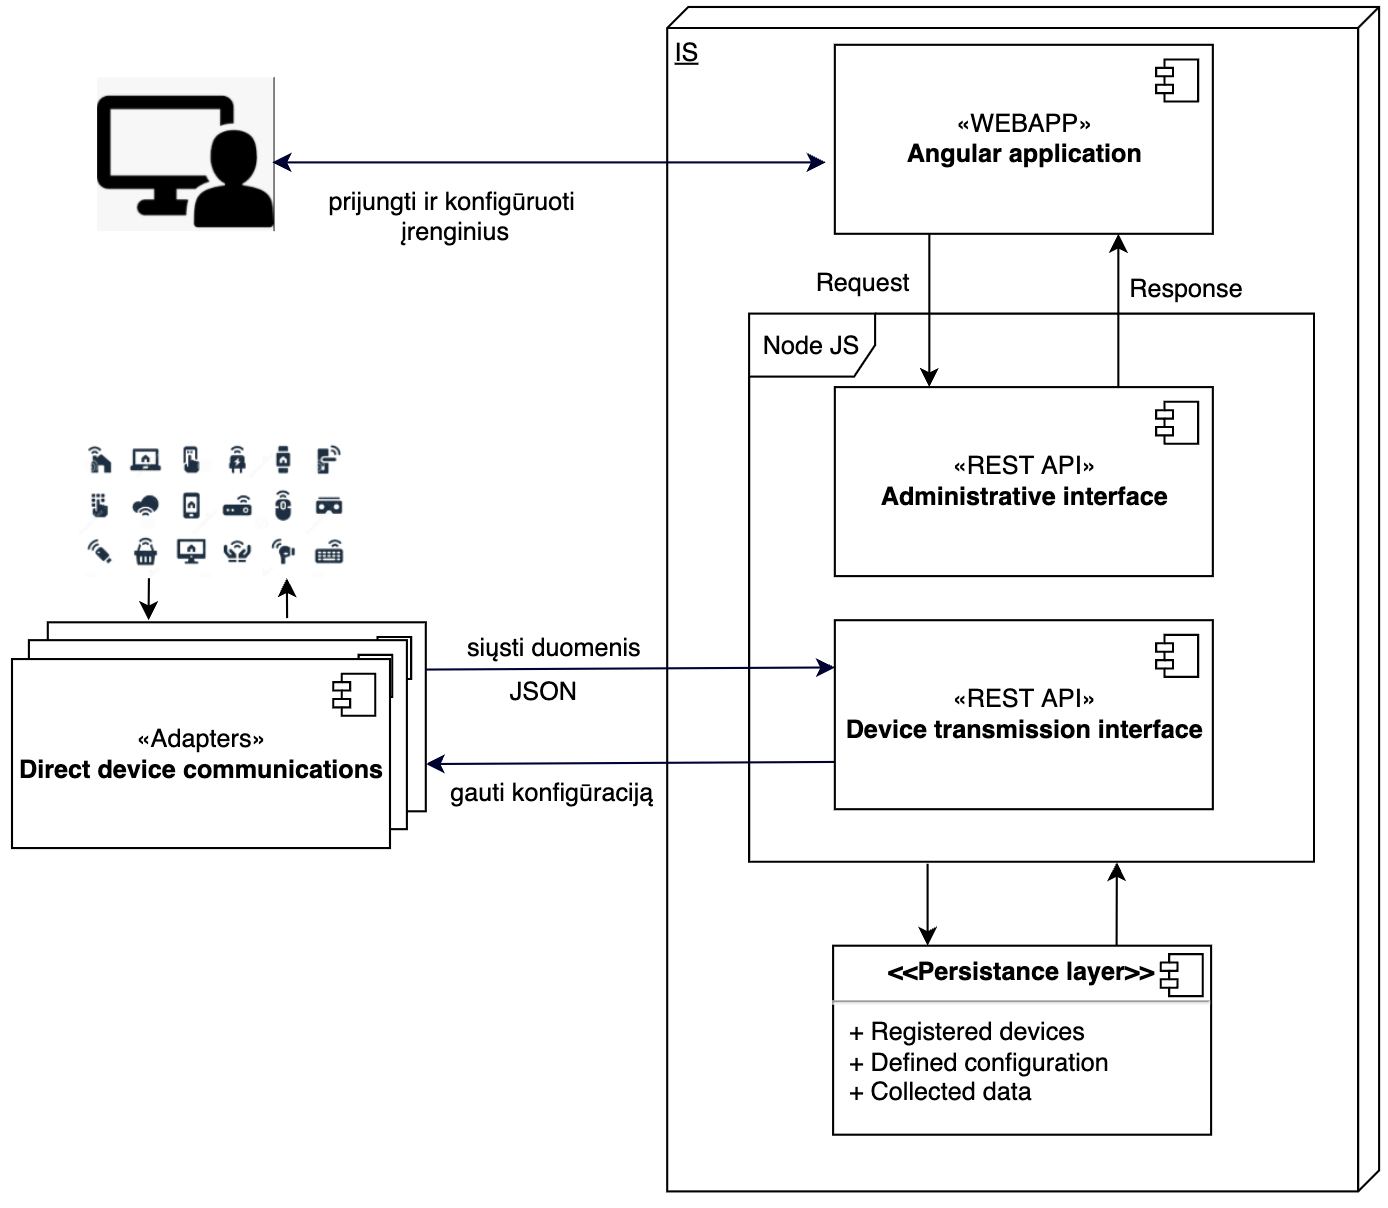
\includegraphics[scale=0.7]{img/vision-s}
    \caption{Sistemos paskirtys}   % Antraštė įterpiama po paveikslėlio
    \label{img:mlp}
\end{figure}

\subsection{Esybės}
\begin{itemize}
\item \emph{Vartotojas(User)} - registruotas sistemos vartotojas. Vartotojas sistemoje turi gebėti pridėti ir konfigūruoti įvairaus tipo įrenginius, peržiūrėti jų siunčiamus duomenis.
\item \emph{Projektas(Project)} - Įrenginių, jų grupių ir juos administruojančių vartotojų visuma. Vienas vartotojas gali dalyvauti daugiau nei viename projekte. Vienas įrenginys(ir jų grupė) egzistuoja tik vieno projekto ribose.
\item \emph{Grupė(Group)} - įrenginių organizavimas į mažesnes logines grupes(vieno projekto kontekste) pagal projekto komandos(vartotojų) apibrėžtą tvarką.
\item \emph{Įrenginys(Device)} - vieną fizinį įrenginį atitinkanti esybė.
Kaip savo atributus turi dinaminę įrenginio siunčiamų duomenų schemą ir vartotojo valdomą prietaiso konfigūraciją.
\item \emph{Valydmo Taisyklė(Control Rule)} - automatizuoto įrenginių valdymo instrukcija.
Kaip savo atributus turi sąrašą sąlygų - sąlygas apibrėžia administratorius, jos tikrina iš nurodytų įrenginių atsiųstus duomenis. Veiksmai(\emph{Actions}) nurodo kaip ir kokiems įrenginiams pakeičiama konfigūraciją, jei joje apibrėžtos sąlygos yra patenkintos.
\end{itemize}

\subsection{Klasių diagrama}
\begin{figure}[H]
    \centering
    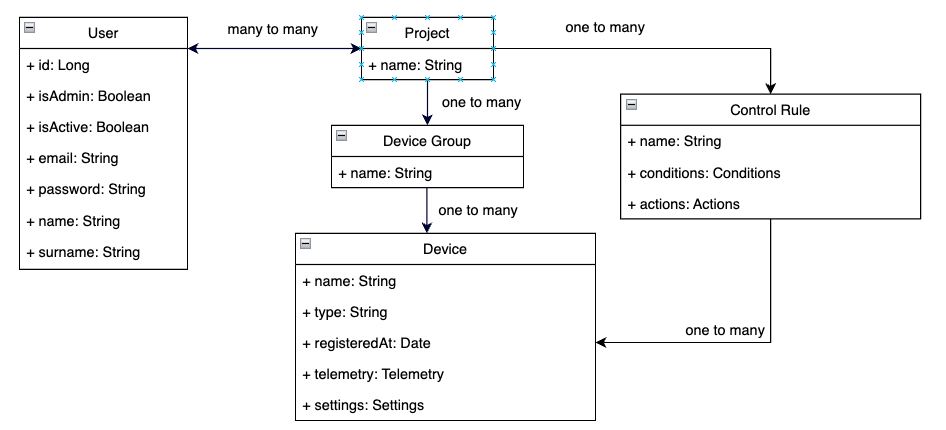
\includegraphics[scale=0.5]{img/class-diagram-iot-v1}
    \caption{Sistemos esybių sąryšiai}
    \label{img:mlp}
\end{figure}

\subsection{Panaudojimo atvejai}

\begin{figure}[H]
  \centering
  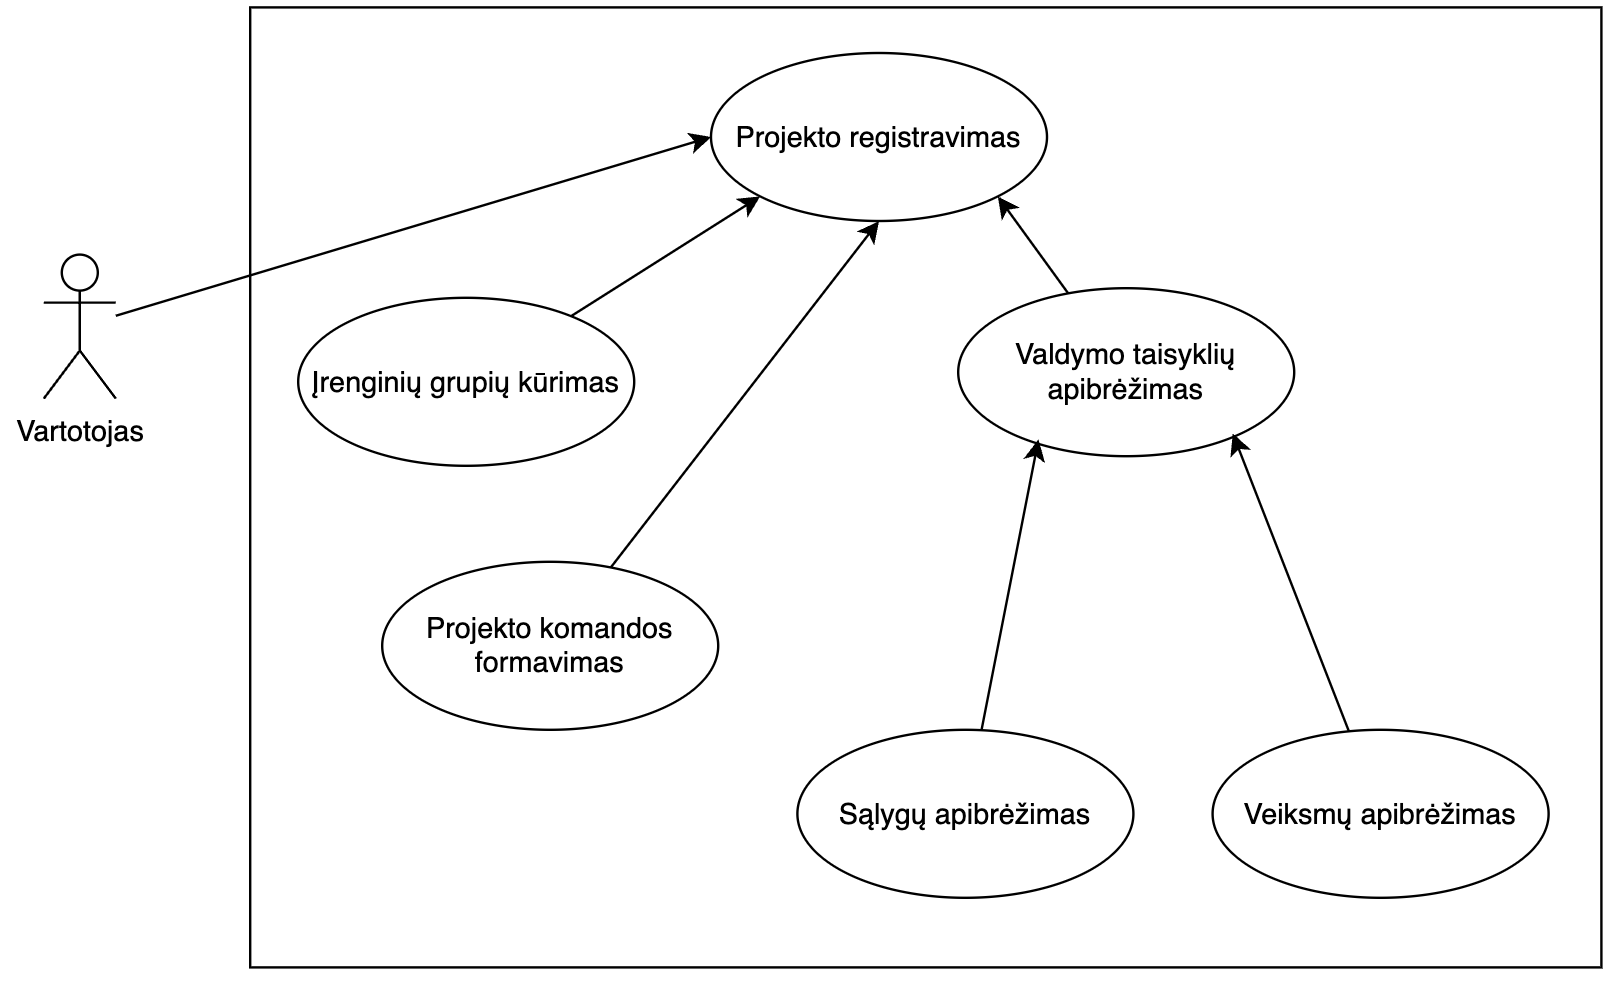
\includegraphics[scale=0.6]{img/UC-projects}
  \caption{Projekto administravimas}
  \label{img:mlp}
\end{figure}

%
% UC create project
%
\begin{tabular}{  l  p{10cm}  p{15cm} }
\toprule
\textbf{Pavadinimas}
& \textbf{Projekto registravimas} \\
\midrule

Aprašymas
& Sukuriamas naujas, tuščias projektas įrenginių registravimui, stebėjimui ir valdymui. \\

\hline
Aktorius    
& Vartotojas \\

\hline
Prieš sąlyga
& - \\

\hline
Vykdymo eiga    
& 1. Įvedama projekto informacija \\

\hline
Po sąlyga
& Vartotojas automatiškai tampa projekto administratoriumi \\
\bottomrule
\end{tabular}

\hfill \break

%
% UC define control rule
%
\begin{tabular}{  l  p{10cm}  p{15cm} }

\toprule
\textbf{Pavadinimas}
& \textbf{Valdymo taisyklių apibrėžimas} \\
\midrule

Aprašymas
& Valdymo taisyklių apibrėžimas \\

\hline
Aktorius    
& Vartotojas \\

\hline
Prieš sąlyga
& 1. Vartotojas dalyvauja projekte ir suteiktos teisės. \\

\hline
Vykdymo eiga    
& 1. Apibrėžiamos sąlygos \\
& 2. Apibrėžiami veiksmai \\
\bottomrule
\end{tabular}

\hfill \break

%
% UC define condition
%
\begin{tabular}{  l  p{10cm}  p{15cm} }

\toprule
\textbf{Pavadinimas}
& \textbf{Sąlygų apibrėžimas} \\
\midrule

Aprašymas
& Valdymo taisyklės sąlygų apibrėžimas. Valdymo taisyklė fiksuoja nurodytų įrenginių duomenis ir tikrina ar jų reikšmės atitinka nurodytas sąlygas. Jei sąlygos tenkinamos - taisyklė pritaikoma \\

\hline
Aktorius    
& Vartotojas \\

\hline
Prieš sąlyga
& 1. Vartotojas dalyvauja projekte ir suteiktos teisės \\
& 2. Projekte egzistuoja įrenginys(-iai) su apibrėžta duomenų schema ir konfigūracija \\

\hline
Vykdymo eiga    
& 1. Pasirenkamas projekte regisruotas įrenginys \\
& 2. Pasirenkama įrenginio duomenų schemos nuoroda \\
& 3. Pasirenkamas sąlygos operatorius \\
& 4. Įvedama skaitinė reikšmė, kuri yra lyginiama su įrenginio duomenų reikšme \\

\hline
Alternatyvūs veiksmai
& 1. Vartotojas gali apibrėžti norimą skaičių sąlygų vienoje taisyklėje \\
& 2. Vartotojas gali panaikinti pasirinką sąlygą iš taisyklės \\
\bottomrule
\end{tabular}

\hfill \break

\begin{tabular}{  l  p{10cm}  p{15cm} }

\toprule
\textbf{Pavadinimas}
& \textbf{Valdymo taisyklės veiksmų apibrėžimas} \\
\midrule

Aprašymas
& Valdymo taisyklės veiksmų apibrėžimas. Jei visos taisyklėje apibrėžtos sąlygos yra patenkintos, sistema atlieka veiksmus - keičia nurodytų įrenginių konfigūraciją pagal taisyklėje nurodytas reikšmes \\

\hline
Aktorius    
& Vartotojas \\

\hline
Prieš sąlyga
& 1. Vartotojas dalyvauja projekte ir suteiktos teisės \\
& 2. Projekte egzistuoja įrenginys(-iai) su apibrėžta duomenų schema ir konfigūracija \\

\hline
Vykdymo eiga    
& 1. Pasirenkamas projekte regisruotas įrenginys \\
& 2. Pasirenkama įrenginio konfigūracijos schemos nuoroda \\
& 3. Įvedama nauja konfigūracijos parametro reikšmė \\

\hline
Alternatyvūs veiksmai
& 1. Vartotojas gali apibrėžti norimą skaičių veiksmų vienoje taisyklėje \\
& 2. Vartotojas gali panaikinti pasirinką veiksmą iš taisyklės. \\
\bottomrule
\end{tabular}

%
% UC manage project team
%
\begin{tabular}{  l  p{10cm}  p{15cm} }

\toprule
\textbf{Pavadinimas}
& \textbf{Projekto komandos formavimas} \\
\midrule

Aprašymas
& Vartotojų pridėjimas ir šalinimas iš projekto \\

\hline
Aktorius    
& Vartotojas \\

\hline
Prieš sąlyga
& 1. Vartotojas dalyvauja projekte ir suteiktos teisės. \\

\hline
Vykdymo eiga    
& 1. Į projektą pridedamas kitas egzistuojantis sistemos vartotojas. \\
& arba \\
& 1. Vartotojas pašalinamas iš projekto \\
& arba \\
& 1. Vartotojas palieka projektą \\
\bottomrule
\end{tabular}

\begin{figure}[H]
  \centering
  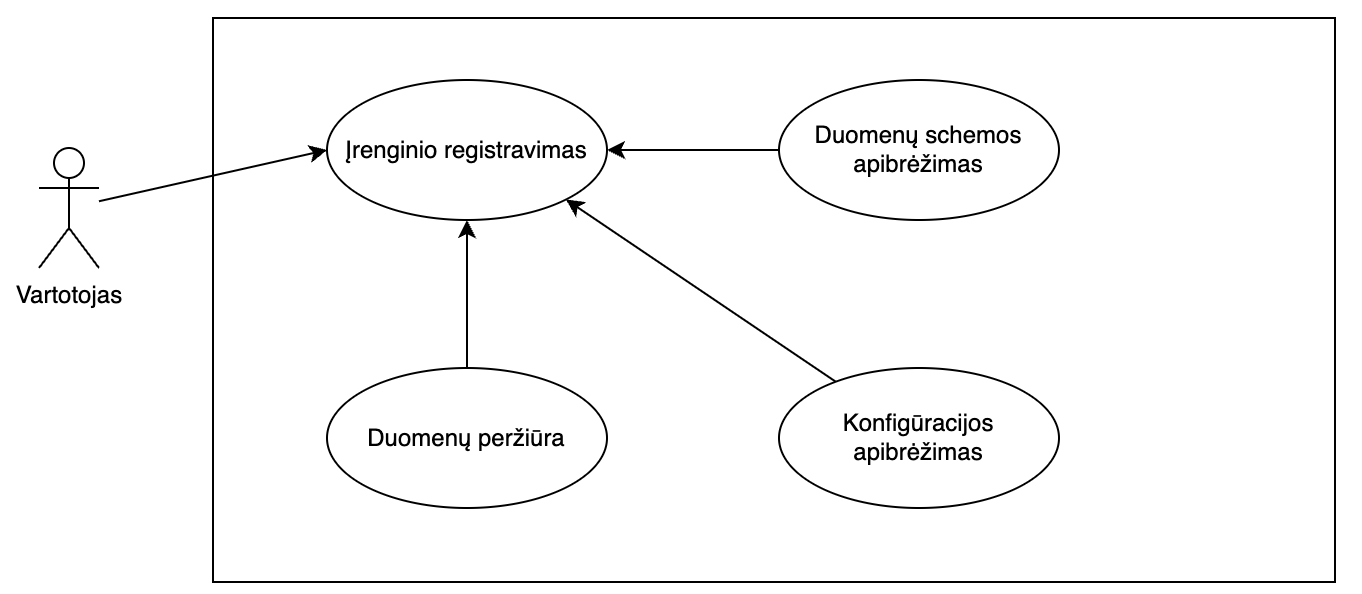
\includegraphics[scale=0.7]{img/UC-devices}
  \caption{Įrenginio administravimas}
  \label{img:mlp}
\end{figure}

%
% Device UC device registration
%
\begin{tabular}{  l  p{10cm}  p{15cm} }

\toprule
\textbf{Pavadinimas}
& \textbf{Įrenginio registravimas} \\
\midrule

Aprašymas
& Naujo įrenginio sistemoje registravimas \\

\hline
Aktorius    
& Vartotojas \\

\hline
Prieš sąlyga
& 1. Vartotojas dalyvauja projekte ir suteiktos teisės. \\
& 2. Projekte sukurta bent viena įrenginių grupė. \\

\hline
Vykdymo eiga    
& 1. Nurodoma įrenginio informacija \\
& 2. Aprašoma duomenų schema \\
& 3. Aprašoma konfigūracija \\
\bottomrule
\end{tabular}
  
\hfill \break

%
% Device UC data review
%
\begin{tabular}{  l  p{10cm}  p{15cm} }

\toprule
\textbf{Pavadinimas}
& \textbf{Duomenų peržiūra} \\
\midrule

Aprašymas
& Įrenginio siunčiamų duomenų peržiūra \\

\hline
Aktorius    
& Vartotojas \\

\hline
Prieš sąlyga
& 1. Vartotojas dalyvauja projekte ir suteiktos teisės. \\
& 2. Esama įrenginių, kurie siunčia savo duomenis į sistemą. \\

\hline
Vykdymo eiga    
& 1. Įrenginio duomenys peržiūrimi laiko/duomenų grafike \\
\bottomrule
\end{tabular}
  
\hfill \break

\begin{tabular}{  l  p{10cm}  p{15cm} }

\toprule
\textbf{Pavadinimas}
& \textbf{Duomenų schemos apibrėžimas} \\
\midrule

Aprašymas
& Duomenų schema priskirta įrenginiui aprašo kaip sistema nuskaitys įrenginio siučiamus duomenis. \\

\hline
Aktorius    
& Vartotojas \\

\hline
Prieš sąlyga
& 1. Vartotojas dalyvauja projekte ir suteiktos teisės. \\
& 2. Projekte egzistuoja įrenginys(-iai) \\

\hline
Vykdymo eiga    
& 1. Nurodomas duomenų pavadinimas sistemos aplinkoje. \\
& 2. Įvedama nuoroda nusakanti kelią iš kurio bus nuskaityta reikšmė. \\

\hline
Alternatyvūs veiksmai
& 1. Vartotojas gali apibrėžti pasirinktą skaičių nuorodų \\

\bottomrule
\end{tabular}

\hfill \break

\begin{tabular}{  l  p{10cm}  p{15cm} }

\toprule
\textbf{Pavadinimas}
& \textbf{Sąlygų apibrėžimas} \\
\midrule

Aprašymas
& Įrenginio konfigūracijos apibrėžimas \\

\hline
Aktorius    
& Vartotojas \\

\hline
Prieš sąlyga
& 1. Vartotojas dalyvauja projekte ir suteiktos teisės. \\
& 2. Projekte egzistuoja įrenginys(-iai) \\

\hline
Vykdymo eiga    
& 1. Suteikiamas konfigūracijos parametro pavadinimas sistemos viduje \\
& 2. Pasirenkama konfigūracijos parametro tipas(tekstas, skaičius arba loginis) \\
& 3. Įvedama nuoroda nusakanti kelią į kur bus įrašyta reikšmė.  \\
& 4. Įvedama/nustatoma parametro reikšmė \\

\hline
Alternatyvūs veiksmai
& 1. Vartotojas gali apibrėžti pasirinktą skaičių konfigūracijos parametrų \\

\bottomrule
\end{tabular}

\begin{figure}[H]
  \centering
  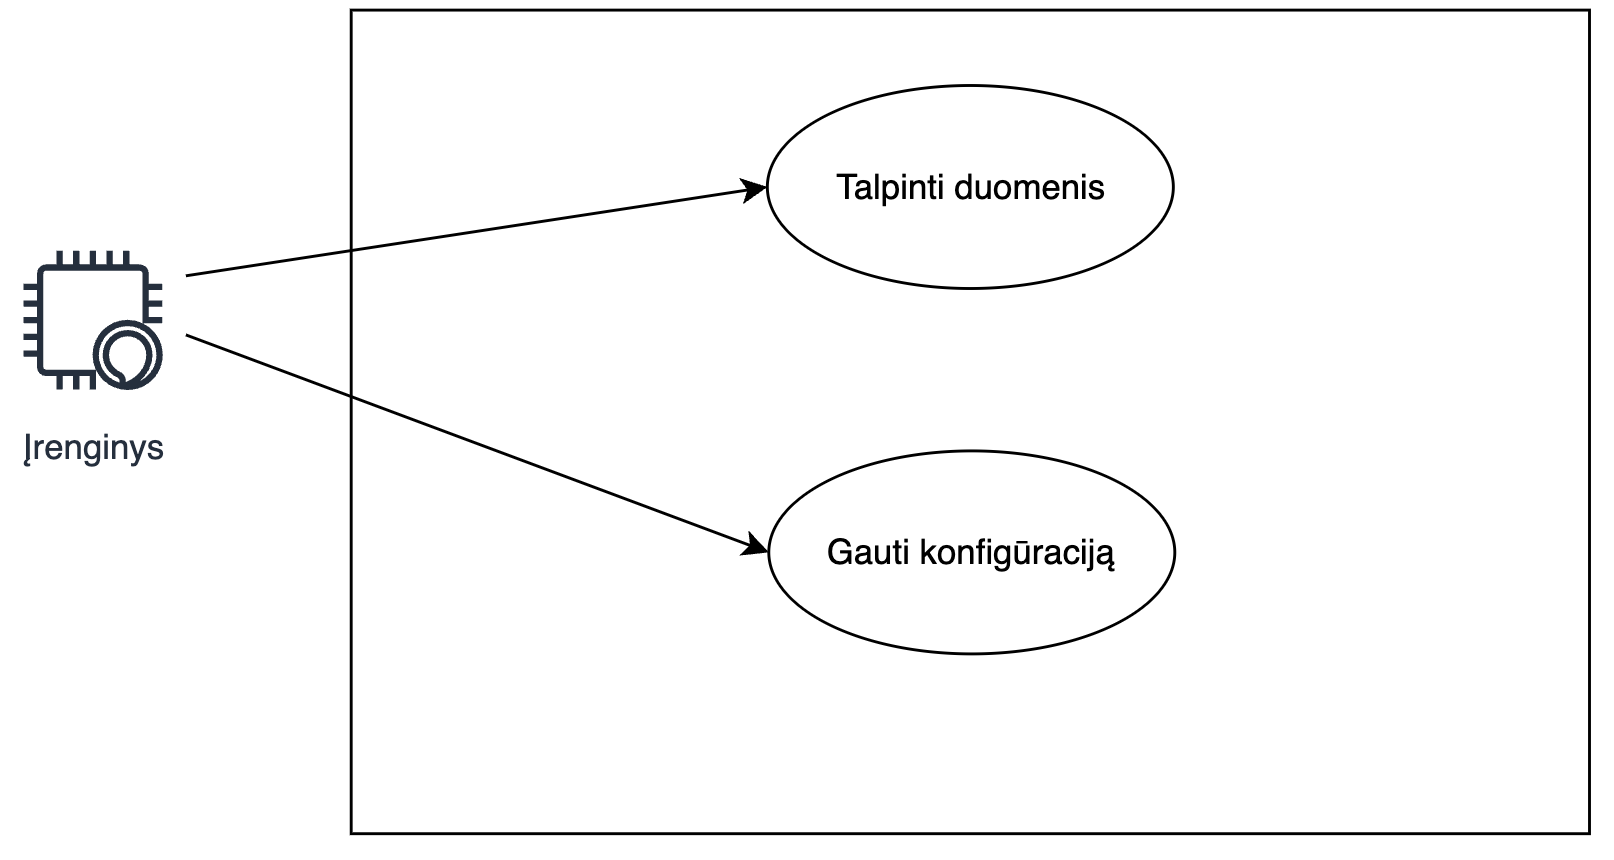
\includegraphics[scale=0.6]{img/UC-device}
  \caption{Įrenginio ir sistemos komunikacija}
  \label{img:mlp}
\end{figure}

\begin{tabular}{  l  p{10cm}  p{15cm} }

\toprule
\textbf{Pavadinimas}
& \textbf{Duomenų talpinimas} \\
\midrule

Aprašymas
& Sistemoje registruotas ir atitinkamai sukonfigūruotas įrenginys siunčia duomenis į sistemą \\

\hline
Aktorius
& Įrenginys \\

\hline
Prieš sąlyga
& 1. Įrenginys registruotas sistemoje \\
& 2. Įrenginys turi apibrėžta duomenų schemą \\

\hline
Vykdymo eiga
& 1. Iškviečiamas duomenų fiksavimo WEB servisas \\
& 2. Atsiustas duomenų paketas filtruojamas pagal įrenginiui apibrėžtą duomenų schemą, saugojami tik nurodyti laukai \\

\bottomrule
\end{tabular}

\hfill \break

%
% UC renew config
%
\begin{tabular}{  l  p{10cm}  p{15cm} }

\toprule
\textbf{Pavadinimas}
& \textbf{Konfigūracijos atnaujinimas} \\
\midrule

Aprašymas
& Konfigūracija leidžia koreguoti/valdyti įrenginio būseną, atliekamą funkciją ir kitas galimas konkretaus įrenginio parinktis \\

\hline
Aktorius    
& Įrenginys \\

\hline
Prieš sąlyga
& 1. Įrenginys registruotas sistemoje \\

\hline
Vykdymo eiga
& 1. Iškviečiamas konfigūracijos naujinimo WEB servisas \\
& 2. Tikrinimos valdymo taisyklės, galinčios koreguoti besikreipiančio įrenginio konfigūraciją \\
& 3. Į įrenginį išsiunčiama naujausia konfigūracija \\

\hline
Schema
&
\begin{minipage}{.5\textwidth}
  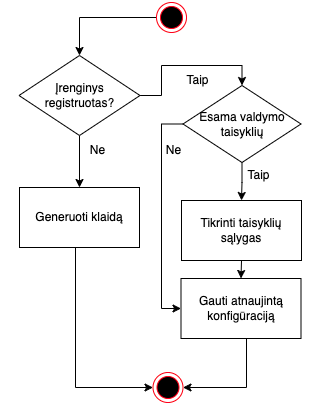
\includegraphics[scale=0.6]{img/flowchart-config}
\end{minipage} \\

\bottomrule
\end{tabular}


\subsection{Įrenginio konfigūracijos formos}
Iš skritingų įrenginių siunčiamos informacijos kiekis ir struktūra gali būti skirtinga, reikalingas būdas priklausomai nuo įrenginio fiksuoti perdavimo metu gautus duomenis.
Lygiai tas pat principas galioja ir konfigūracijos parametrams.
Įrenginio peržiūros ir registravimo languose pridedame dinamines formas kuriose vartotojas apibrėžia kaip iš įrenginio gauti duomenys bus fiksuojami ir kokios struktūros konfigūracija bus siunčiama į prietaisą, šiam paprašius atnaujinti konfigūraciją.
Šie apibrėžimai nėra vartotoja pasirinkimo laisvė - jie priklauso nuo atitinkamo įrenginio specifikacijos. Tokiu būdu, varotojas atlieka sistemos ir įrenginio derinimą.
\begin{figure}[H]
    \centering
    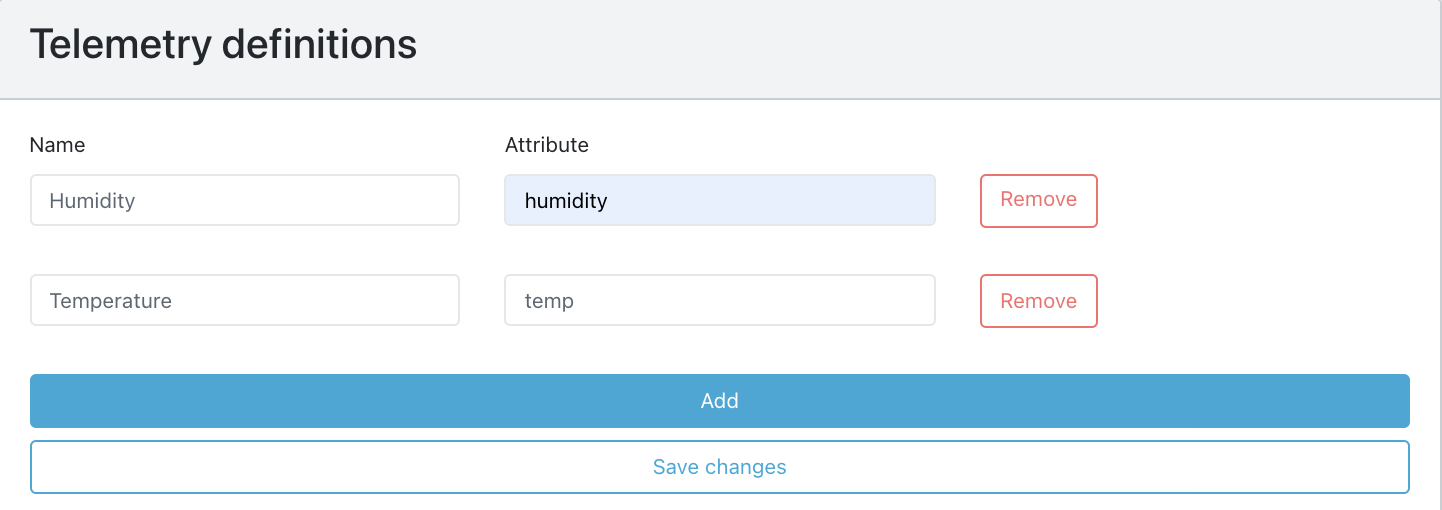
\includegraphics[scale=0.5]{img/telemetry-form}
    \caption{Vartotojas apibrėžia kaip nuskaityti įrenginio siunčiamus duomenis}
    \label{img:mlp}
\end{figure}

\subsection{Įrenginio peržiūros ir grupavimo langai}

Pavyzdyje matome įrenginių grupių sąrašo langą. Viršutiniame kampe nurodoma kurio projekto kontekste vartotojas šiuo metu yra.
Šalia yra išsiskleidžiantis sąrašas kurio elementai - visi projektai kuriuose prisijungęs vartotojas dalyvauja.
Grupių pavadinimai projekte yra pasirenkamaimi laisvai, taigi projekto komanda gali nuspresti kaip bus atliekamas skirstymas.
Kiekvienos grupė savyje turi jai priklausančių įrenginių sąrašą.

\begin{figure}[H]
    \centering
    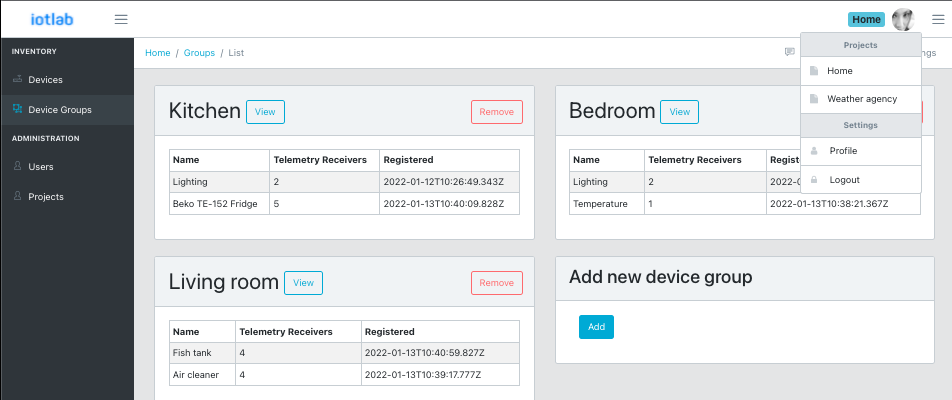
\includegraphics[scale=0.5]{img/device-groups-results}
    \caption{Įrenginių grupės namo kambariams}   % Antraštė įterpiama po paveikslėlio
    \label{img:mlp}
\end{figure}

Įrenginio peržiūros ir konfigūracijos lange galima matyti iš įrenginio atsiūstų duomenų grafikus.
Konfigūruoti kaip gauti duomenys yra nuskaitomi ir kokie nustatymai galioja užregistruotam įrenginiui. 

\begin{figure}[H]
    \centering
    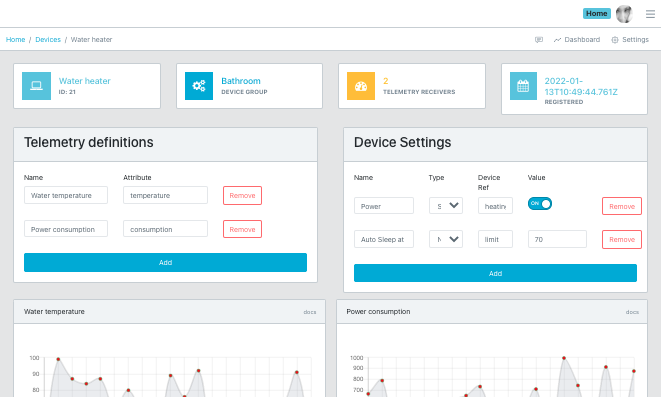
\includegraphics[scale=0.6]{img/device-settings-results}
    \caption{Vieno įrenginio konfigūracija ir duomenų peržiūra}   % Antraštė įterpiama po paveikslėlio
    \label{img:mlp}
\end{figure}

\subsection{Automatizuoto valdymo konfigūracijos langas}
\begin{figure}[H]
  \centering
  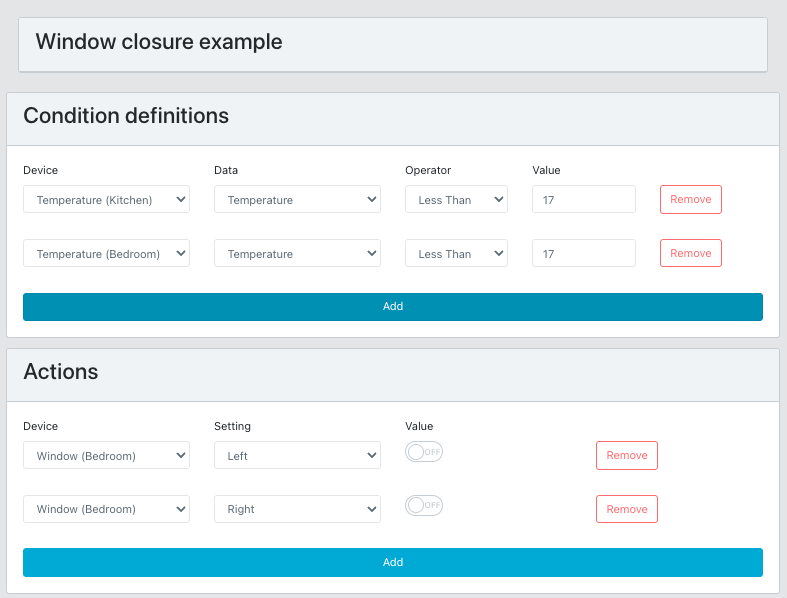
\includegraphics[scale=0.6]{img/window-closure-example}
  \caption{Valdymo taisyklės aprašas: Sąlygos ir veiksmai}   % Antraštė įterpiama po paveikslėlio
  \label{img:mlp}
\end{figure}

Valydmo taisyklės pavyzdyje pateikiamas scenarijus - dviejuose kambariuose fiksuojama temperatūra. Jei abu sensoriai praneša, kad temperatūra žemesnė, nei nurodyta sąlygoje, vykdomi taisyklėje 
apibrėžti veiksmai. Languose esantys valdikliai uždaro langus. \emph{Sąlygos} aprašas nurodo įrenginį, jo siunčiamų duomenų nuorodą, loginį operatorių palyginimui atlikti ir reikšmę, su kuria yra lyginimas paskutinis įrenginio atsiųstas duomenų vienetas. \emph{Veiksmas} aprašomas nurodant įrenginį, jo konfigūracijos lauką ir naują jo reikšmę.
Vienoje taisyklėje galima apibrėžti daugiau nei vieną sąlygą ir daugiau nei vieną veiksmą. Taisyklės veiksmai vykdomi jei visos apibrėžtos sąlygos yra patenkintos.

\section{Technologijos ir įgyvendinimas}
\subsection{Technologijos}
\begin{figure}[H]
    \centering
    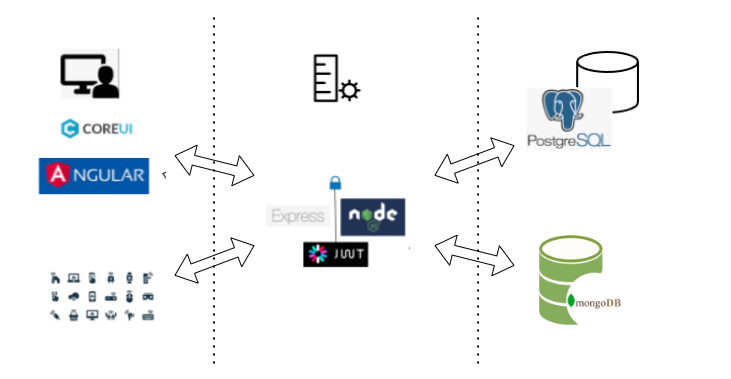
\includegraphics[scale=0.6]{img/arch-schema-v1}
    \caption{Sistemos komponentai}   % Antraštė įterpiama po paveikslėlio
    \label{img:mlp}
\end{figure}

\begin{itemize}
  \item \emph{Angular} - TypeScript programavimo kalbos karkasas WEB vartotojo sąsajos kūrimui.
  \item \emph{Core UI} - naudojimui paruoštų Angular komponentų ir CSS stilių rinkinys.
  \item \emph{Node JS} - serverio programinės įrangos vykdymo aplinka(programavimo kalba - Javscript).
  \item \emph{Express} - biblioteka skirta REST tipo Web servisams kurti.
  \item \emph{JWT} - autentifikacijos biblioteka.
  \item \emph{Postgres SQL} - registruoti įrenginiai, sistemos vartotojai ir įrenginių konfigūracijos saugomos reliacinėje duomenų bazėje.
  \item \emph{Mongo DB} - įrenginių siunčiami duomenys saugojami dokumentinėje duomenų bazėje. \cite{MONGODB, JOBD}
\end{itemize}

\subsection{Vartotojo sąsaja}
\subsubsection{Angular}

Angular yra platforma ir sistema, skirta kurti vieno puslapio kliento programas naudojant HTML ir TypeScript.
Angular parašyta TypeScript programavimo kalba. Jis įgyvendina pagrindines ir pasirenkamas funkcijas kaip „TypeScript“ bibliotekų rinkinį.
Karkaso architektūra remiasi tam tikromis pagrindinėmis sąvokomis. „TypeScript“ bibliotekos sudarančios Angular karkasą vadinamos \emph{Moduliais(Module)}.
Moduliai surenka susijusį kodą į funkcinius rinkinius; programa apibrėžiama modulių rinkiniu.
 
Programa visada turi bent vieną(šakninį) modulį, kuris įgalina įkrovą, o dažnu atveju, Angular aplikacijos turi daug daugiau funkcijų modulių. Jie leidžia programuotojui rašyti modulines programas ir pernaudoti kodą vietoje dublikavimo.
\emph{Komponentai(Component)} apibrėžia rodinius, kurie yra ekrano elementų rinkiniai, kuriuos Angular gali pasirinkti ir modifikuoti pagal kuriamos programos logiką ir duomenis.

Komponentai naudoja \emph{Servisus(Service)}, kurie teikia specifines funkcijas, tiesiogiai nesusijusias su vaizdu, kurį mato vartotojas. Servisai gali būti įtraukti į komponentus kaip priklausomybės, todėl kodas tampa modulinis, pakartotinai naudojamas ir efektyvus.
Kiekvienas komponentas turi sau priskirtą dali HTML teksto dalį kuri atvaizduojama vartotojo sąsajoje, jie vadinami \emph{Šablonais(Template)}.
Šablonas sujungia įprastą HTML su Angular direktyvomis, leidžiančiu modifikuoti HTML prieš pateikiant jį rodyti. Arba keisti matomus duomenis aplikacijos naudojimo metu.

Programos komponentai paprastai apibrėžia daugybę rodinių(\emph{Views}), išdėstytų hierarchiškai. „Angular“ teikia maršrutizatoriaus(\emph{Router}) paslaugą, kuri padės nustatyti naršymo kelius tarp vaizdų. Maršrutizatorius suteikia sudėtingas naršymo naršyklėje galimybes.

\begin{figure}[H]
    \centering
    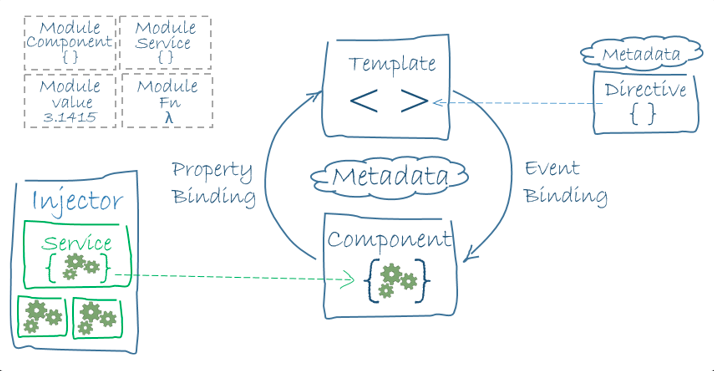
\includegraphics[scale=0.5]{img/angular-schema}
    \caption{Angular konceptas išsidėstymas}   % Antraštė įterpiama po paveikslėlio
    \label{img:mlp}
\end{figure}

Angular aplikacijos kodas yra vykdomas vartotojo kompiuteryje, naudojamos naršyklės Javascript interpretatoriuje.
Taigi galutinis HTML išeities tekstas yra sukuriamas dinamiškai, kliento mašinoje. 
Vartotojo sąsajos prasme, serverio dalis sistemoje yra atsakinga tik už Angular aplikacijos kodo pateikimą statinių failų pavidalu.
Angular \emph{Service} klasės atlieka HTTP kreipinius į sistemos WEB servisą siekiant atlikti prisijungimą prie sistemos arba gauti vartotojo pageidaujamus duomenis.

\subsubsection{Angular Reactive forms}
Tai vienas iš Angular karkaso modulių leidžiančių dirbti su HTML formomis.
Angular reaktyviosios formos laikosi modeliu pagrįsto metodo formų įvesties apdorojimui, kurios vertės laikui bėgant gali būti keičiamos.
Tai taip pat žinoma kaip modeliu pagrįstos formos. Reaktyviosiose formose galime sukurti ir atnaujinti savo paprastą formos įvedimo lauką, naudoti kelis įvedimo elementus grupėje, 
atlikti formos reikšmių validavimą, įdiegti sudėtingesnes formas, dinamiškai pridėti ir šalinti formos įvedimo laukus.

Reaktyviosiose formose naudojamas aiškus ir nekintamas būdas valdyti formos būseną tam tikru momentu. Kai pakeičiame formos būseną, ji grąžina naują būseną, kuri valdo modelių vientisumą tarp pakeitimų.
Naudojant ši modulį, komponento klasėje sukuriame formą atspindintį kintamąjį, kurio pagalbą galima sekti formos būseną. 

Modulio interfeisas susideda iš keleto klasių: \cite{AngularRectiveForms}

\begin{tabular}{  l  p{10cm}  p{15cm} }

\toprule
\textbf{Klasė}
& \textbf{Paskirtis} \\
\midrule

AbstractControl
& Abstrakčioji bazinė klasė formų valdymo klasėms FormControl, FormGroup ir FormArray. Tai suteikia jiems bendrą elgesį ir savybes. \\

\hline
Form Control     
& Tvarko individualaus formos įvedimo lauko reikšmę ir validumą. Tai atitinka HTML formos įvedimo lauką, pvz., <input> arba <select> \\

\hline
Form Group
& Tvarko „AbstractControl“ egzempliorių grupės reikšmę ir įvesties validumą. Grupės ypatybės apima jos antrinius valdiklius(esanšius grupėje). Komponento aukščiausio lygio forma yra FormGroup klasės egzempliorius. \\

\hline
Form Array
& Tvarko skaitiniu būdu indeksuoto AbstractControl egzempliorių masyvą. Ši klasė leidžia vykdomo metu į formą pridėti naujus įvedimo laukus, arba įvedimo laukų grupes.
Naudojantis šia klase galima sukurti dinaminę įvedimo formą, kurios struktūrą iš dalies gali apibrėžti pats vartotojas.\\

\hline
FormBuilder
& Injekcinė paslauga, teikianti gamyklinius valdymo egzempliorių kūrimo metodus. \\

\bottomrule
\end{tabular}

Pateiktame pavyzdyje(7 pav.) matome TypeScript objekto reikšmę ir jį atitinkančą HTML formą. Pasikartojančios eilutės ir saugomos kaip \emph{FormArray} sąrašo nariai.
Vartotojas pasirintinai gali pridėti naują arba pašalintį norimą įvesties eilutę. Kiekviena eilutė savaime priklauso klasei \emph{FormGroup}, kadangi savyje turi keletą įvedimo laukų. 
Kiekvienas įvedimo laukas atspindimas \emph{FormControl} klasės objektu.

\begin{figure}[H]
    \centering
    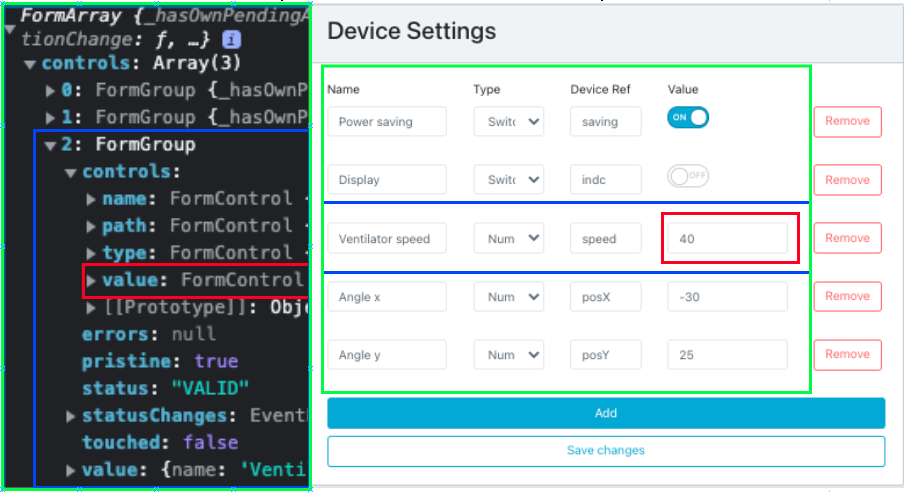
\includegraphics[scale=0.5]{img/reactive-form-example}
    \caption{Dinaminės formos pav.}   % Antraštė įterpiama po paveikslėlio
    \label{img:mlp}
\end{figure}

\subsubsection{Core UI}

Naudojimui paruoštų Angular komponentų ir CSS stilių rinkinys. Tai leidžia pagreintinti grafinės aplikacijos dalies kūrimą.
Kadangi šios sistemos kūrimo metu nėra griežtai aprašytų dizaino reikalavimų, taip pat siekiant supaprastinti vartotojo sąsajos grafinės dalies uždavinius naudojame Core UI siūlomus HTML ir CSS pavydžius:

\begin{itemize}
  \item HTML elementų pozicionavimas ir išdėstymas naršyklės lange.
  \item Spalvų deriniai.
  \item Formų ivedimo laukai, mygtukai, šoninė navigacijos juosta.
  \item Prisijungimo ir navigacijos langai.
\end{itemize}

\subsection{Serverio programinė įranga}

\subsubsection{ER Diagrama}
\begin{figure}[H]
  \centering
  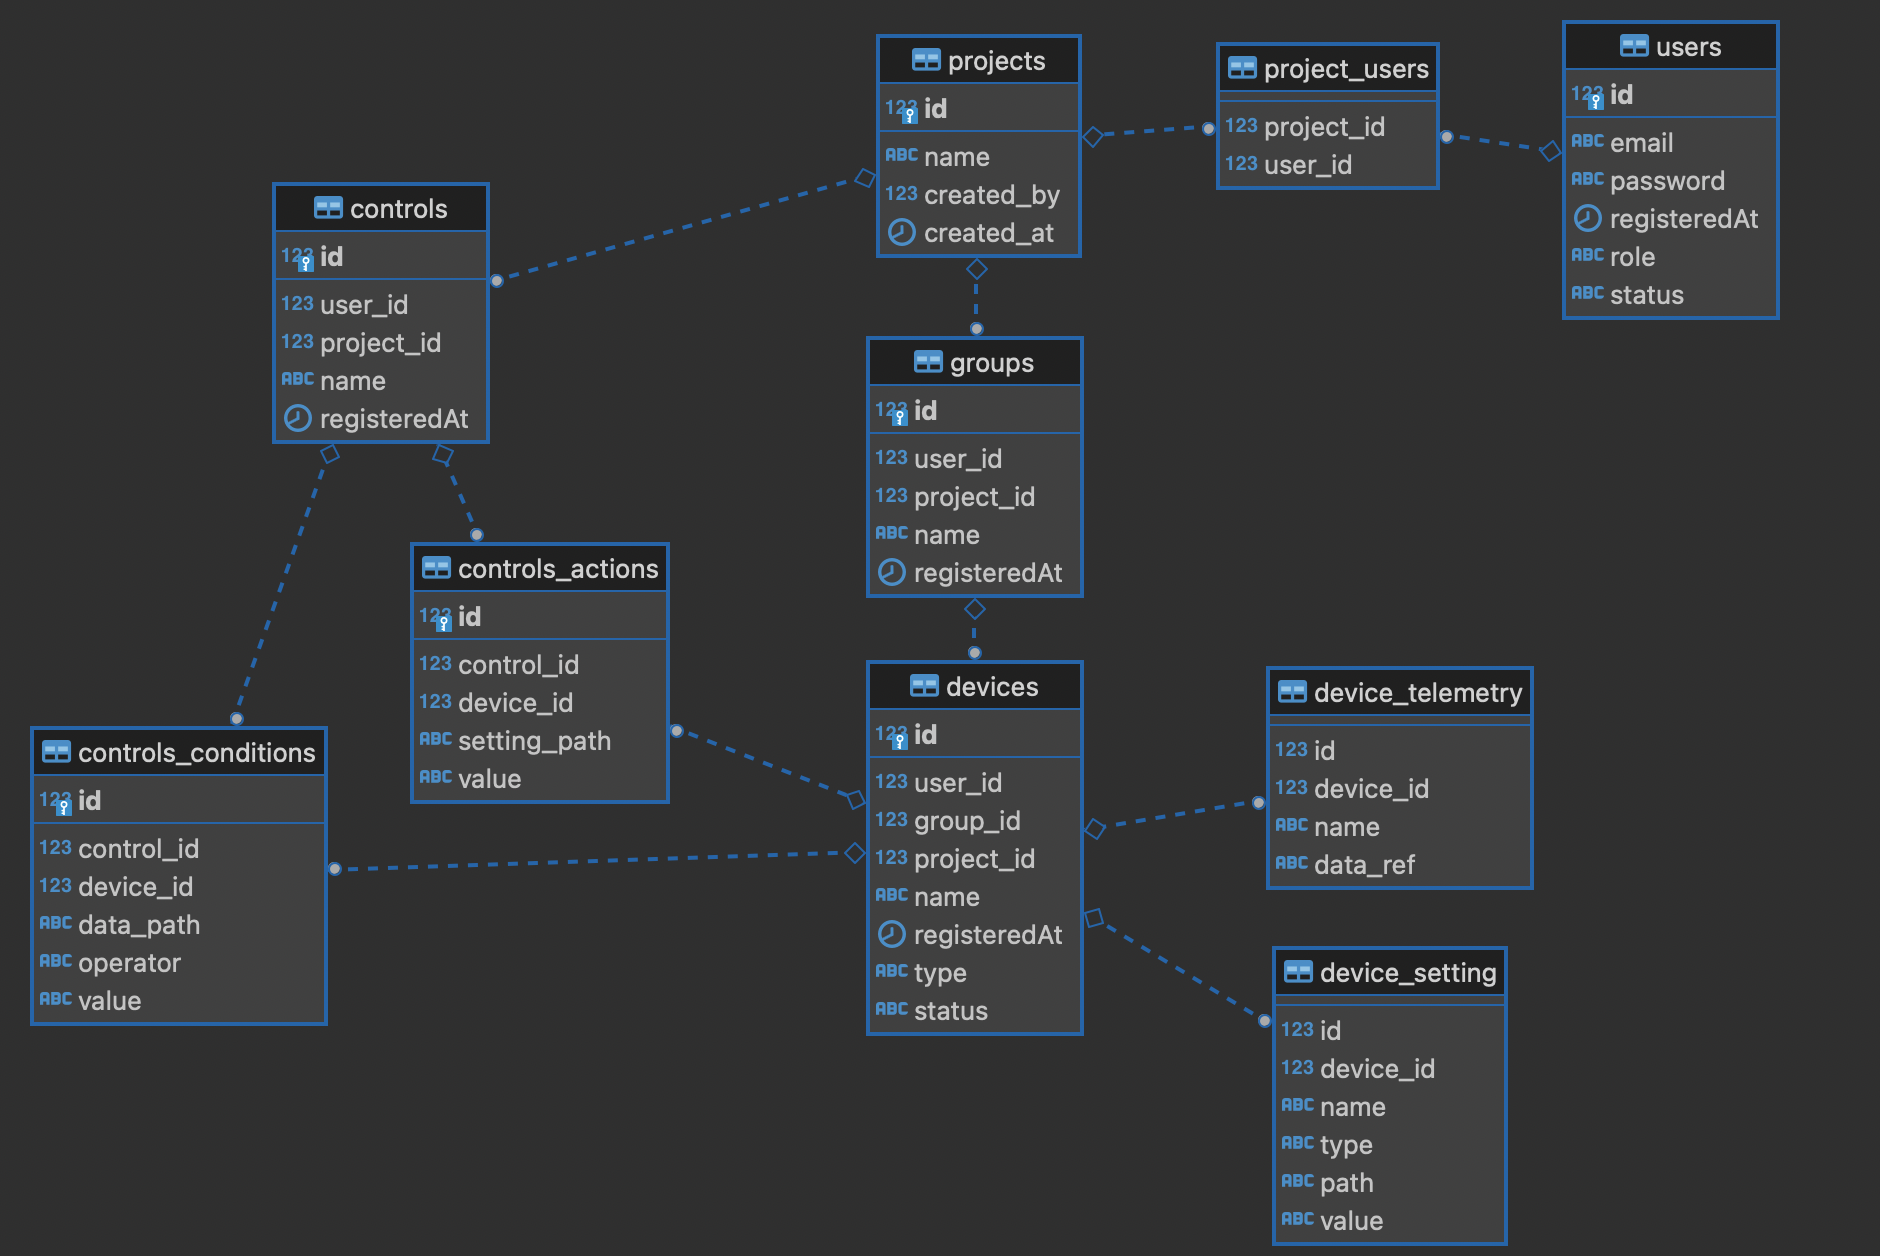
\includegraphics[scale=0.5]{img/er-diagram}
  \caption{RDBMS schema}
  \label{img:mlp}
\end{figure}

\subsubsection{Express}

„Express“ yra populiariausia „Node JS“ biblioteka skirta API ir WEB servisų kūrimui. Express naudojami ir daugelio kitų 
NPM bibliotekų kaip sudedamoji dalis.
Jame numatyti mechanizmai:

\begin{itemize}
\item Nesudėtingai aprašyti serverio maršrutus(\emph{Routes, Endpoints}) ir su jais susieti atitinkamas apdorojimo funkcijas.
\item Pridėti papildomas funkcijas prie vieno resurso arba jų grupės. Tai įgalina moduliarumą, visišką laisvę pasirinti kaip bus vykdoma
užklausų autentifikacija, kokiu formatu į WEB servisą atkeliaus duomenys ir kaip bus suformuotas atsakymas.
\end{itemize}

\begin{lstlisting}[language=Java]
  const express = require('express');
  const app = express();
  app.get('/', (req,res)=>{
    res.send('Hi, your request has been received')
  });

  app.listen(2000, ()=>{
    console.log('listening at http://localhost:2000')
  })
\end{lstlisting}

\subsubsection{Serverio programos stuktūra}

\begin{itemize}
\item \emph{server} - programos įeities taškas.
\item \emph{static} - vartotojo sąsajos statinių failų pateikimas į kliento kompiuterį.
\item \emph{auth} - vartotojo prisijungimo, atsijungimo ir authentifikacijos mechanizmas, paremtas JWT.
\item \emph{config} - programos konfigūracija - duomenų bazės prisijungimo slaptažodžiai. JWT privataus ir viešo rakto reikšmės, WEB serverio portas.
\item \emph{devices, groups, projects, users} - sistemos esybių logika - kiekvienas paketas savyje turi HTTP užklausas apdorančias funkcijas, taip pat generuoja esybei aktualias užklausas į paketą db-connector.
\item \emph{control} - Įrenginių siunčiamų signalų ir duomenų apdorojimas. 
\item \emph{db-connector} - Prisijungimas prie Postgres duomenų bazių valdymo sistemos. \cite{NODEJSDB} 
\end{itemize}

\begin{figure}[H]
    \centering
    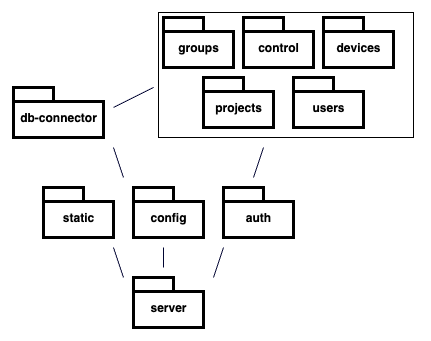
\includegraphics[scale=0.7]{img/local-js-packages}
    \caption{Serverio dalies Node JS paketai}
    \label{img:mlp}
\end{figure}

Pasirinkimas serverio dalį igyvendinti Node JS technologijomis suteikė galimybę rinkis iš daug NPM repositorijose viešai prieinamų 
atviro kodo bibliotekų. Node JS ekosistemoje esama daugybė kiekvienai sistemos daliai įgyvendinti reikalingų bibliotekų.
(Web servisai, autentifikacija, duomenų bazės prieiga). Kita vertus, kai pasirinkimas platus, prieš įtraukiant bibliotekas į projektą svarbu
įsitikinti, kad biblioteka atliks tai ko tikimasi.
Kadangi Node JS bibliotekų repositorijos yra viešos jose galima rasti ir įrankių kurie nebūtinai veiks korektiškai arba yra pritaikyti tik
bendriniams panaudojimo atvejams, nesuteikdami mūsų projektui reikalingo funkcionalumo.

\subsubsection{Autentifikacija naudojant JWT}

JWT(angl. Json web token) yra standartas, apibrėžiantis kompaktišką ir savarankišką būdą, kaip saugiai perduoti informaciją tarp kliento ir serverio kaip JSON objektą.
Dėl kompaktiško dydžio žetonus lengva perduoti per URL, POST parametrą arba HTTP antraštėje.
Be to, kadangi jie yra savarankiški, juose yra visa reikalinga informacija apie vartotoją, todėl duomenų bazės nereikia užduoti daugiau nei vieną kartą.
JWT esančia informacija galima pasitikėti, nes ji yra skaitmeniniu būdu pasirašyta naudojant slaptą arba viešųjų / privačių raktų porą. \cite{JWT}

\begin{enumerate}
\item Registruotas vartotojas pateikia prisijungimo užklausą.
\item Jei vartotojas registruotas sistemoje ir paiekia teisingą slaptažodį, jam sugeneruojamas naujas JWT. 
\item JWT siunčiamas į vartotojo kompiuterį ir išsaugomas naršyklės sesijos atmintyje.
\item Kiekviena duomenų užklausą į WEB servisą siunčiama kartu su šiuo JWT. Serveris, prieš įvykdydamas užklausą patikrina žetono validumą ir galiojimo laiką.
\item Jei pirmieji žingsinai įvykdomi sėkmingai, WEB serviso metodai vartotojui prieinami.
\end{enumerate}

\begin{figure}[H]
    \centering
    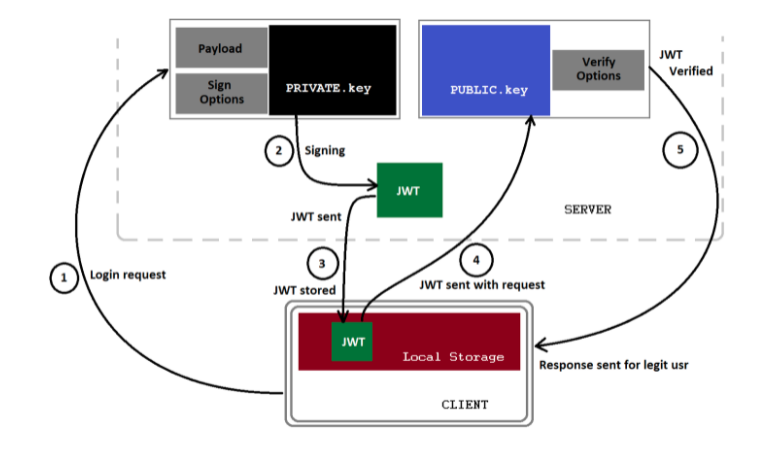
\includegraphics[scale=0.5]{img/jwt-flow}
    \caption{JWT autentifikacijos schema}   % Antraštė įterpiama po paveikslėlio
    \label{img:mlp}
\end{figure}

\sectionnonum{Išvados}

\begin{enumerate}
\item
Informacinė sistema yra tinkama skirtingų tipų ir paskirties įrenginių administravimui ir valdymui.
Suprojektuotas ir realizuotas sprendimas leidžia vartotojams apibrėžti, kokie duomenys ir konfigūracija priskiriami kiekvienam prietaisui.

\item Angular karkaso ir Core UI bibliotekos kombinacija pagreitino ir supaprastino vartotojo sąsajos programavimo darbus.
\emph{Angular Reactive Forms} taikymas palengvino dinaminių įvedimo formų kūrimą,
o \emph{Core UI} elementai leido greitai įgyvendinti patrauklią vartotojo sąsają.

\item Pasirinkimas naudoti \emph{Node JS} serverio pusėje suteikė galimybę naudotis atviro kodo \emph{NPM} bibliotekomis.
\textbf{postgres}, \textbf{mongodb} - prisijungimui į duomenų bazes, \textbf{express} - WEB serviso realizacijai, \textbf{passport-jwt} - authentifikacijai.
\emph{Node JS} bendruomenė yra didelė, bibliotekų skaičius lenkia kitas programavimo kalbas, gausu informacijos internete.
Dėl šių priežasčių, buvo galima daugiau dėmesio sutelkti į informacinės sistemos algoritmų kūrimą, o ne į techninius uždavinius.

\item Documentinė \emph{MongoDB} duomenų bazė skirta prietaisų duomenims laikyti užtikrina greitą duomenų saugojimą,
kadangi, skirtingai nei reliacinėse duomenų bazėse nevykdomi išorinių raktų ir duomenų schemos tikrinimai.

\item Ateityje atsiradus poreikui, \emph{MongoDB} gali būti horizontaliai plečiama į keletą serverių naudojantis \emph{Sharding} galimybėmis.

\item Tolimesniam vystymui galima svarstyti duomenų analitikos, anomalijų atpažinimo, vizualizacijos,
valdymo taisyklių validavimo, papildomų protokolų palaikymo sprendimus.
\end{enumerate}

\sectionnonum{Conclusions}
\begin{enumerate}
\item Informational system is capable of administating and managaing IoT devices of a different kinds and purposes.
Planned and implemented solution allows users to define themselves what data schema and configuration values are applicable for every device.

\item Angular framework and Core UI template collection has reduced frontend delivery time for a good measure.
Angular Reactive Forms allowed to easily develop dynamic user forms.
Core UI elements gave interface attractive appearance out of the box.

\item Node JS as a backend implementation language gave access to large number of open source \emph{NPM} packages. 
\textbf{postgres}, \textbf{mongodb} - connections to databases, \textbf{express} - http web server, \textbf{passport-jwt} - authentication.
Node JS has large and active community, available package and library counts exceeds any other modern programming language.
It is easy to find documentation and information on the net.
These reasons made technical objectives a bit easier and let developer focus more on informational system features.

\item Document type Mongo DB responsible for collected device data storage ensures high data throughput because of the swift nature of Mongo DB technology.
As opposed to relational databases, Mongodb queries does not perform any foreign key checks, neither data schema validation.

\item Usage of Mongo DB leaves horizontal scaling optional available through the feature of Sharding.

\item Further development considerations include data analytics, detection of anomalies, data visualisation, rule contradiction validation,
and additional device protocol support.
\end{enumerate}

\printbibliography[heading=bibintoc] % Literatūros šaltiniai aprašomi
% bibliografija.bib faile. Šaltinių sąraše nurodoma panaudota literatūra,
% kitokie šaltiniai. Abėcėlės tvarka išdėstoma tik darbe panaudotų (cituotų,
% perfrazuotų ar bent paminėtų) mokslo leidinių, kitokių publikacijų
% bibliografiniai aprašai (šiuo punktu pasirūpina LaTeX). Aprašai pateikiami
% netransliteruoti.

\appendix  % Priedai
% Prieduose gali būti pateikiama pagalbinė, ypač darbo autoriaus savarankiškai
% parengta, medžiaga. Savarankiški priedai gali būti pateikiami kompiuterio
% diskelyje ar kompaktiniame diske. Priedai taip pat vadinami ir numeruojami.
% Tekstas su priedais siejamas nuorodomis (pvz.: \ref{img:mlp}).

%\section{Niauroninio tinklo struktūra}
%\begin{figure}[H]
%  \centering
%    \includegraphics[scale=0.5]{img/MLP}
%    \caption{Paveikslėlio pavyzdys}
%    \label{img:mlp}
%\end{figure}
%
%
%\section{Eksperimentinio palyginimo rezultatai}
%% tablesgenerator.com - converts calculators (e.g. excel) tables to LaTeX
%\begin{table}[H]\footnotesize
%  \centering
%  \caption{Lentelės pavyzdys}
%  {\begin{tabular}{|l|c|c|} \hline
%    Algoritmas & $\bar{x}$ & $\sigma^{2}$ \\
%    \hline
%    Algoritmas A  & 1.6335    & 0.5584       \\
%    Algoritmas B  & 1.7395    & 0.5647       \\
%    \hline
%  \end{tabular}}
%  \label{tab:table example}
%\end{table}

\end{document}
